\documentclass{beamer}

\setbeamertemplate{navigation symbols}{}
\usecolortheme{spruce}

%Information to be included in the title page:
\title{REFRACT\\Update presentation}
\author{Carlos Vigil Vásquez}
\institute{$\mu$Platypus Lab, CABD. Sevilla, Spain.}
\date{15 of November, 2022}

\begin{document}

\frame{\titlepage}

\begin{frame}{Introduction}{ACE1}
	\begin{columns}
		\begin{column}{0.5\linewidth}
			\begin{figure}
				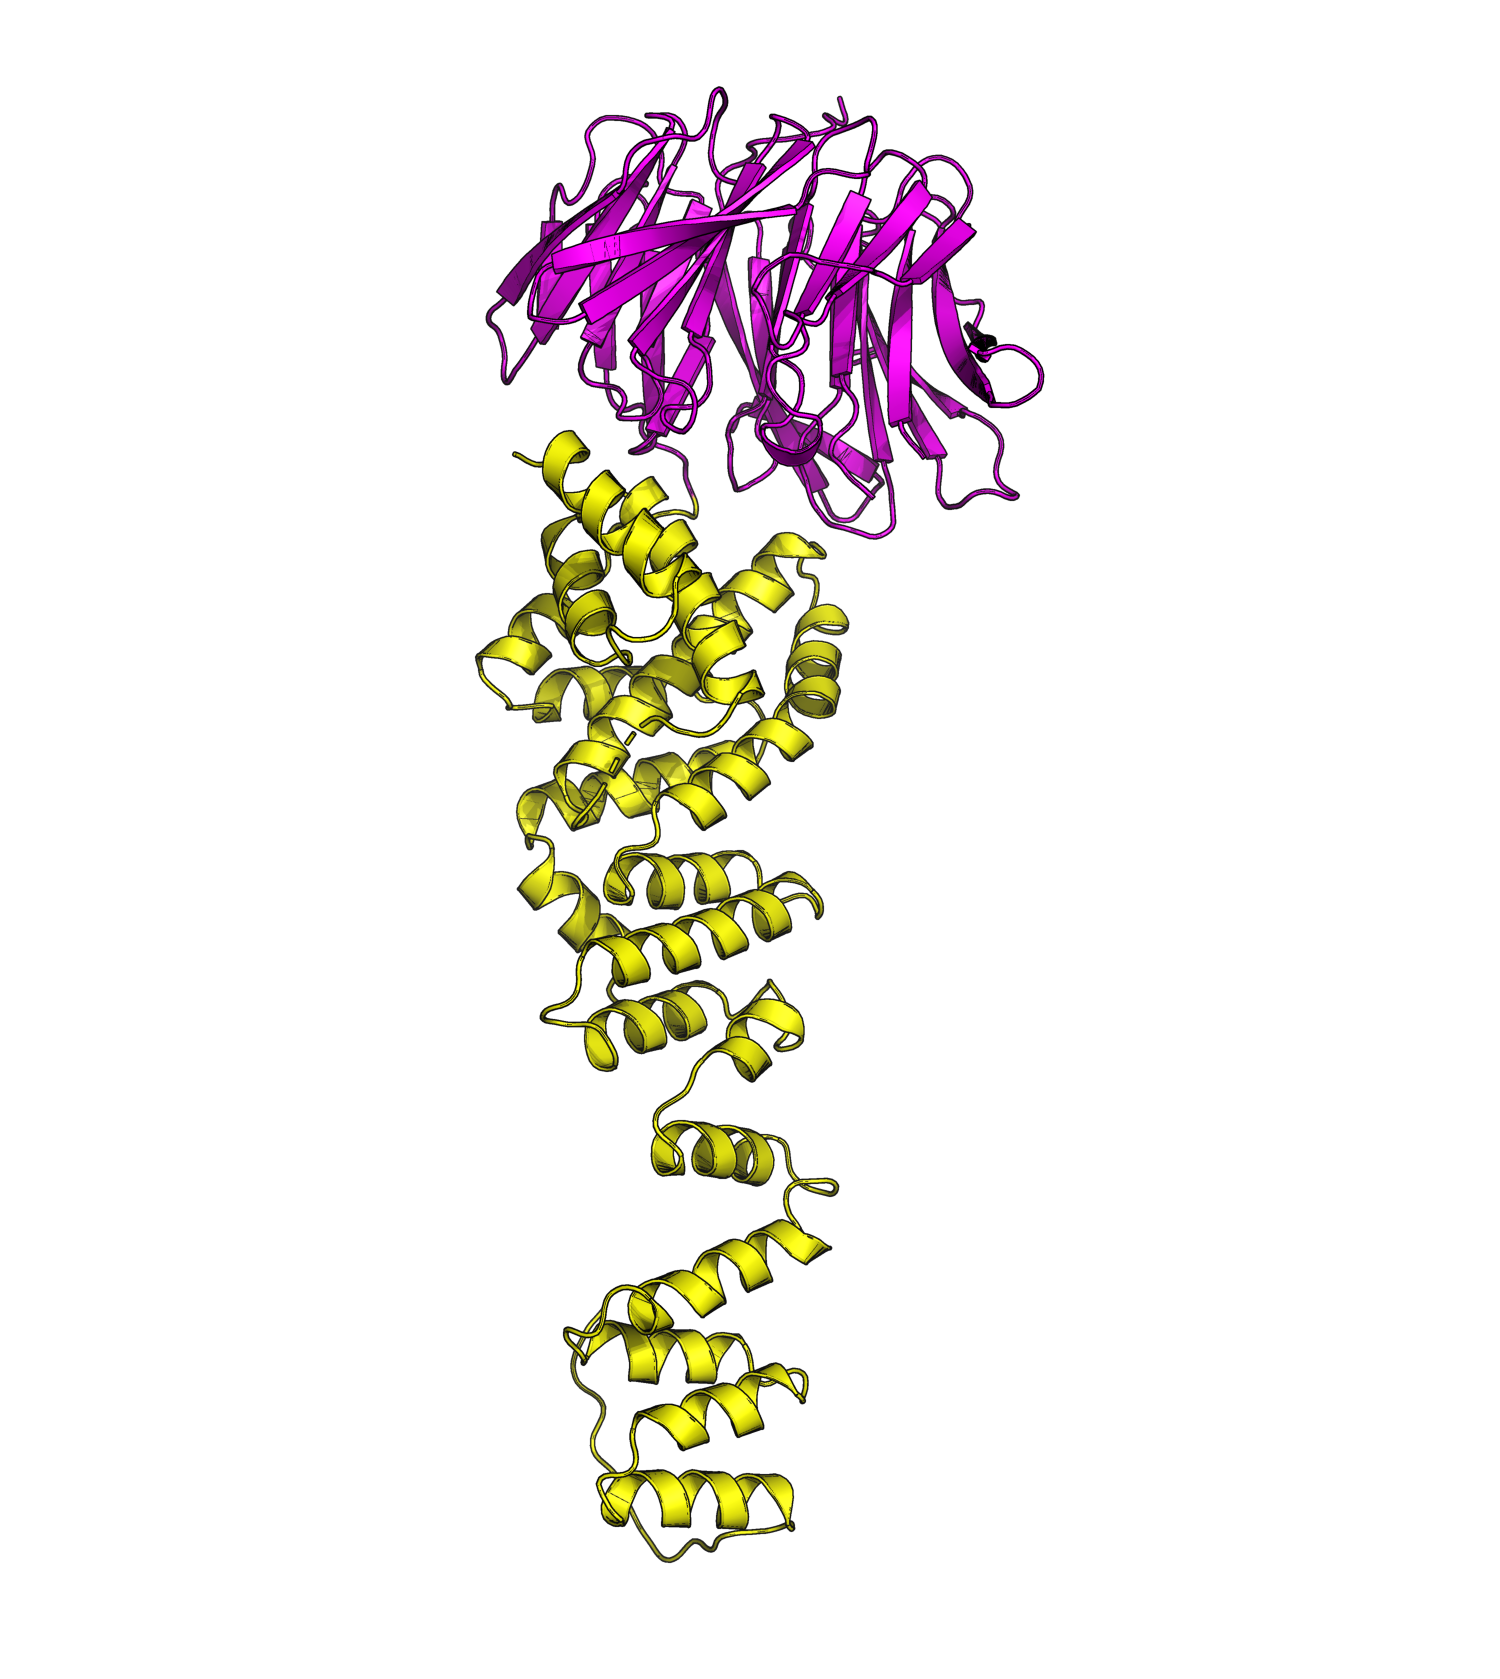
\includegraphics[width=\linewidth]{figures/ACE1_example.png}
				\caption{ACE-1 yeast protein Sec13/31}
			\end{figure}
		\end{column}
		\begin{column}{0.5\linewidth}
			\begin{itemize}
				\item Structural proteins, e.g., nuclear pores \pause
				\item $\beta$ propeller + $\alpha$-solenoid \pause
				\item Head, trunk \& tail \pause
				\item \textbf{$\downarrow$ Conservation signal from amino acid sequence}
				\item \textbf{$\downarrow$ Conservation signal from structural alignment}
			\end{itemize}
		\end{column}
	\end{columns}
\end{frame}

\begin{frame}{Results}{\texttt{Foldseek} optimization}
	\center{Can we improve the understanding of this ACE1-like proteins?}
\end{frame}

\begin{frame}{Results}{\texttt{Foldseek} optimization}
	Use global structural alignment as a proxy,\pause \ 
	then refine interesting cases with local structural alignment.\pause

	\bigskip

	\begin{proof}[Methodology]
		Fast-search with \texttt{Foldseek}, then refine with \texttt{MOMA2}
	\end{proof}

\end{frame}

\begin{frame}{Results}{\texttt{Foldseek} optimization}
	Use \textcolor{red}{global structural alignment as a proxy,} then refine interesting cases with local structural alignment.

	\bigskip

	\begin{proof}[Methodology]
		\textcolor{red}{Fast-search with \texttt{Foldseek},} then refine with \texttt{MOMA2}
	\end{proof}

\end{frame}

\begin{frame}{Results}{\texttt{Foldseek} optimization}
	\center{Can \texttt{Foldseek} find ACE1-like proteins?}
\end{frame}

\begin{frame}{What is \texttt{Foldseek}?}{\texttt{Foldseek} optimization}
	\texttt{Foldseek} is a novel structural alignment tool that ''enables \textbf{fast and sensitive} comparisons of large structure sets.\pause \ It reaches \textbf{sensitivities similar to state-of-the-art}\pause \ structural aligners while being \textbf{four to five orders of magnitude faster}''\footnote[1]{\scriptsize{\textit{Foldseek: fast and accurate protein structure search}, 10.1101/2022.02.07.479398}}.
\end{frame}

\begin{frame}{Results}{\texttt{Foldseek} optimization}
	Optimized \texttt{Foldseek}'s parameters for ACE1 protein search:\pause
	\begin{itemize}
		\item Grid-search optimization \pause 
		\item \texttt{Foldseek} parameters \textit{sensibility} and \textit{k-mer size} \pause 
		\item Complete PDB database \pause
	\end{itemize}

	\bigskip

	\textbf{Objective:} Maximize performance based in finding target proteins with same UniProt accession code
\end{frame}

\begin{frame}{Results}{\texttt{Foldseek} optimization}
	\begin{figure}
	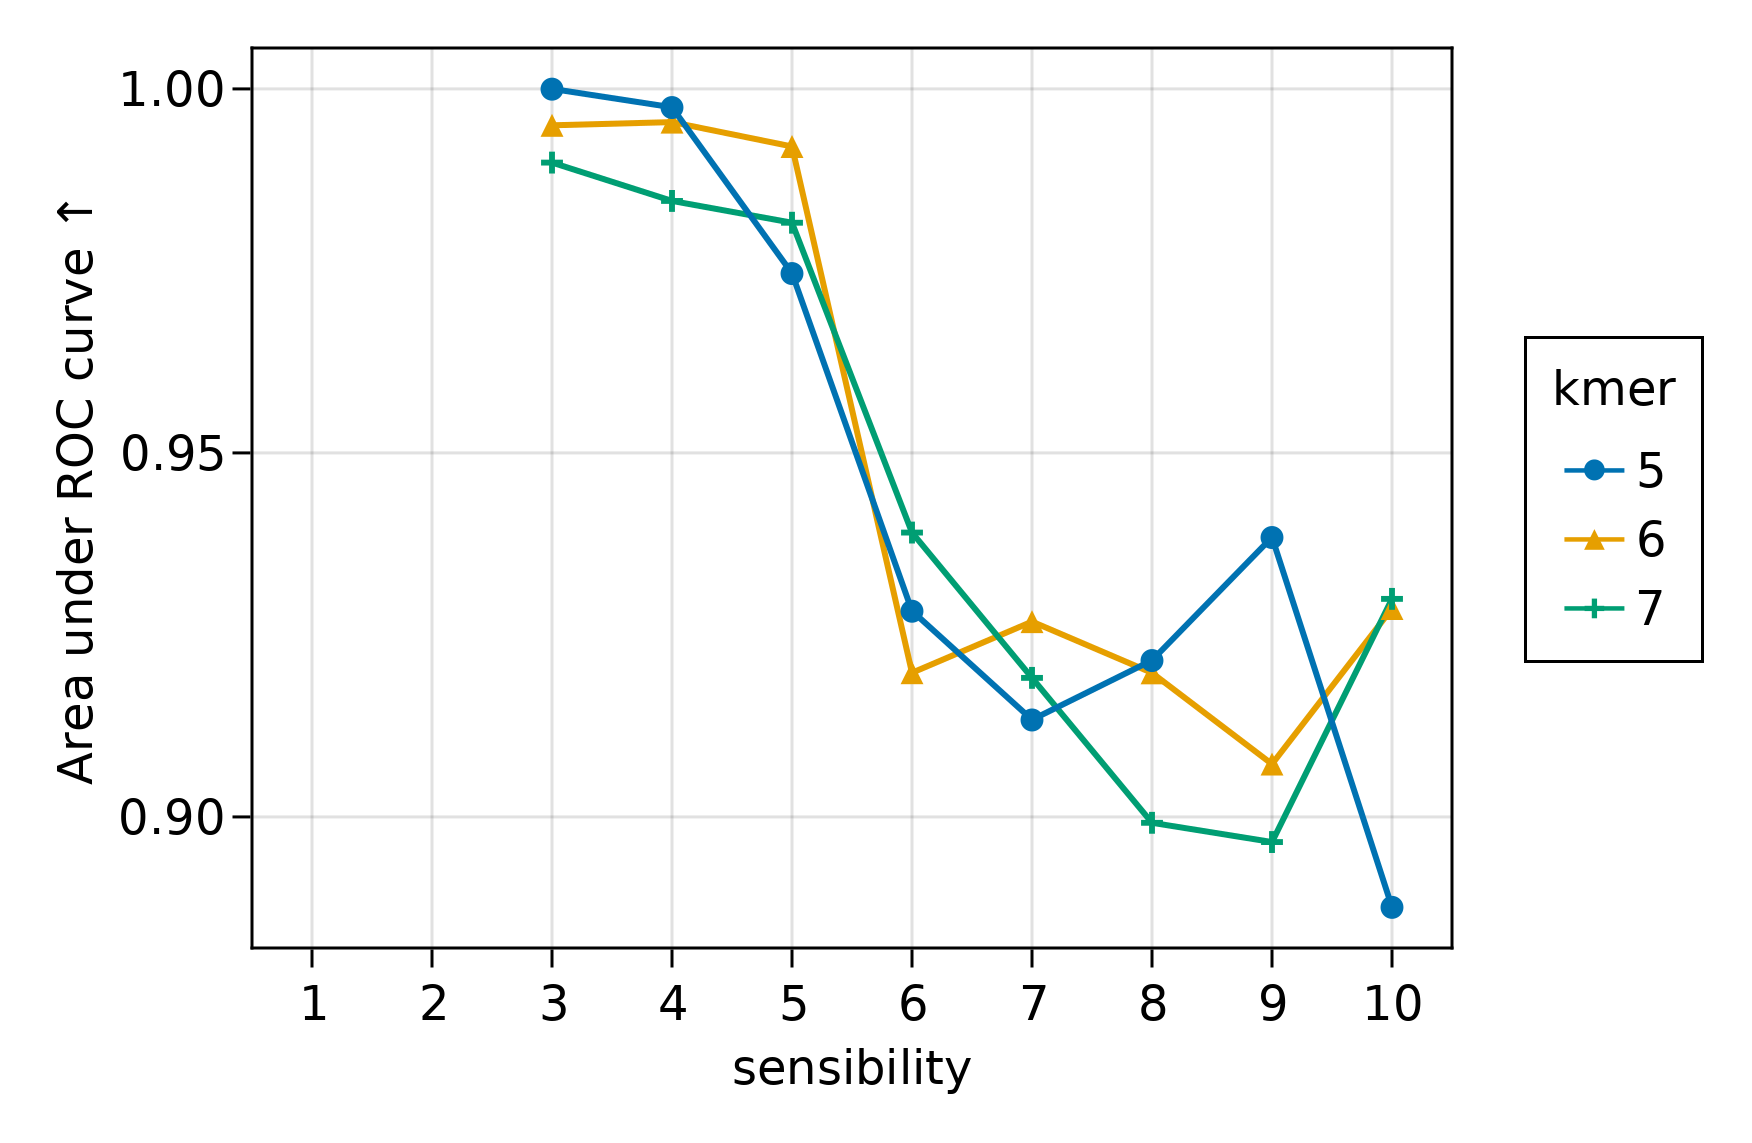
\includegraphics[width=0.8\linewidth]{figures/AuROC_optimization.png}
	\caption{Parameter optimization for ACE1-like protein search based in AuROC}
	\end{figure}
\end{frame}

\begin{frame}{Results}{\texttt{Foldseek} optimization}
	\begin{figure}
	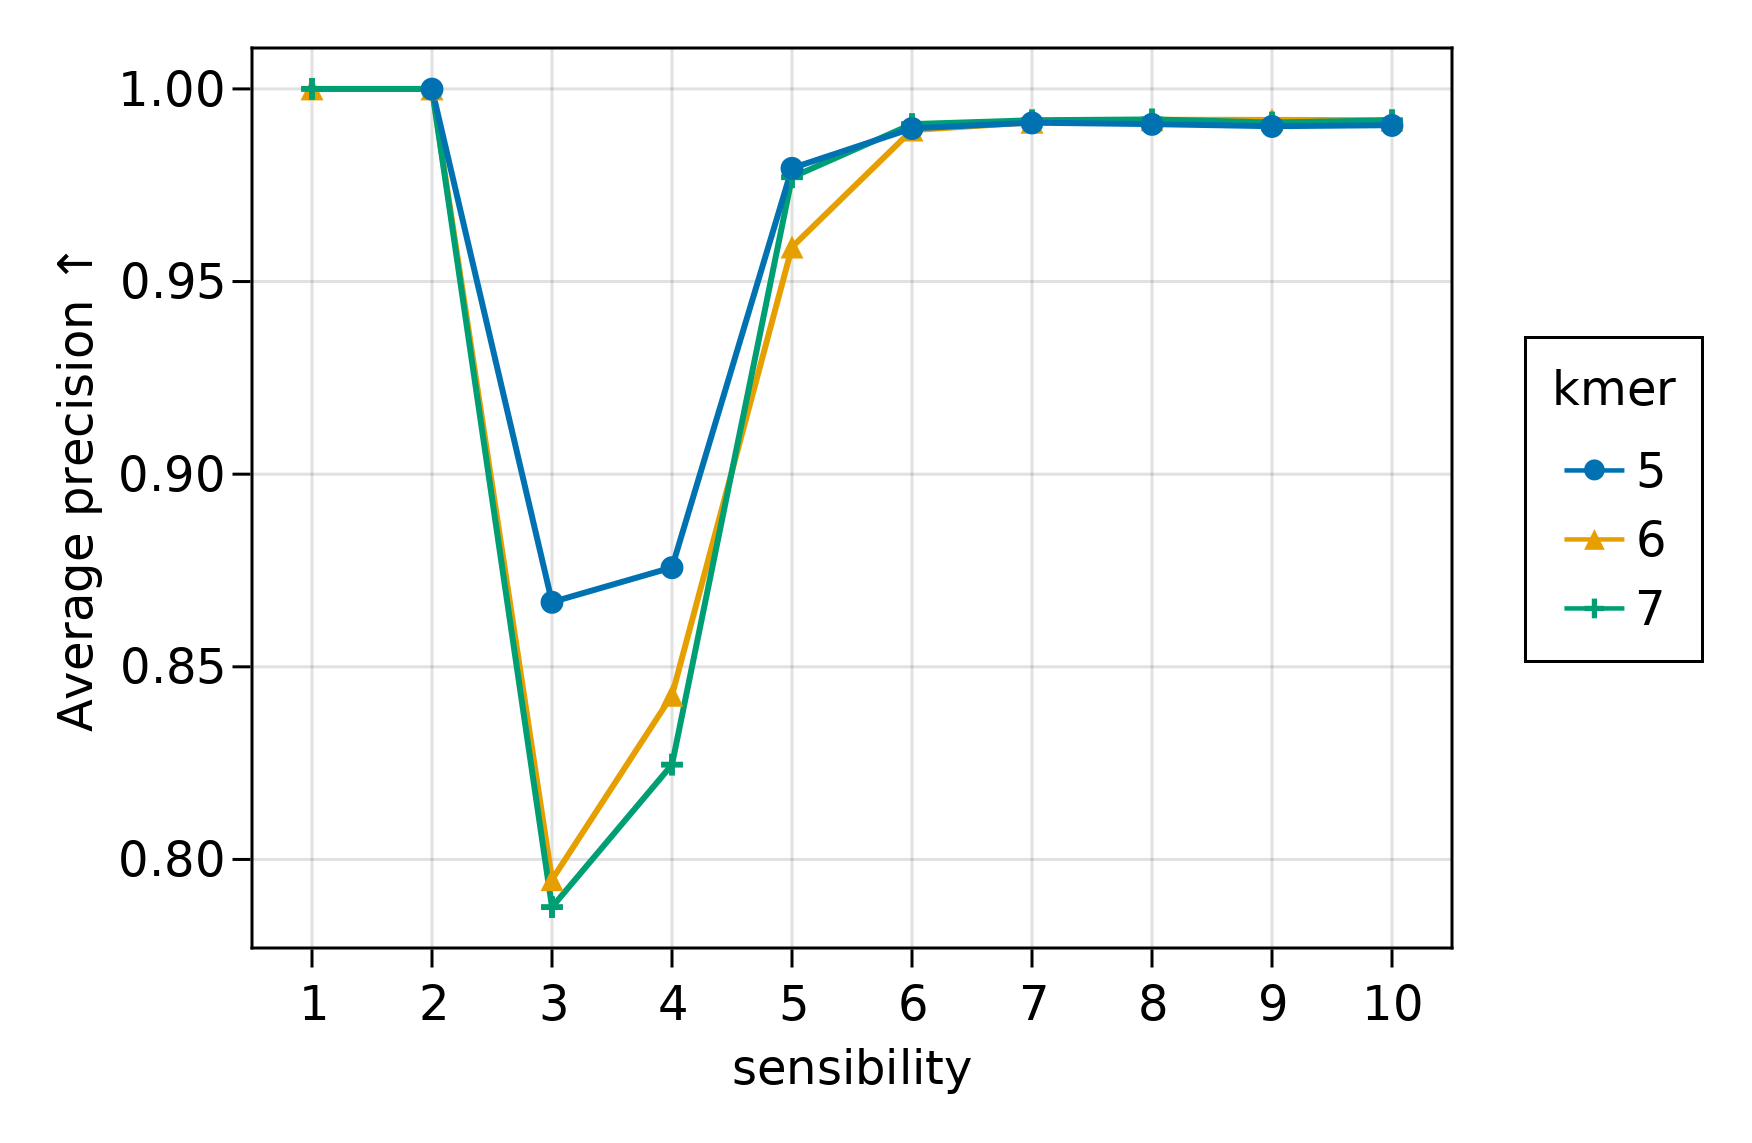
\includegraphics[width=0.8\linewidth]{figures/AuPRC_optimization.png}
	\caption{Parameter optimization for ACE1-like protein search based in AuPRC}
	\end{figure}
\end{frame}

\begin{frame}{Results}{\texttt{Foldseek} optimization}
	\begin{figure}
	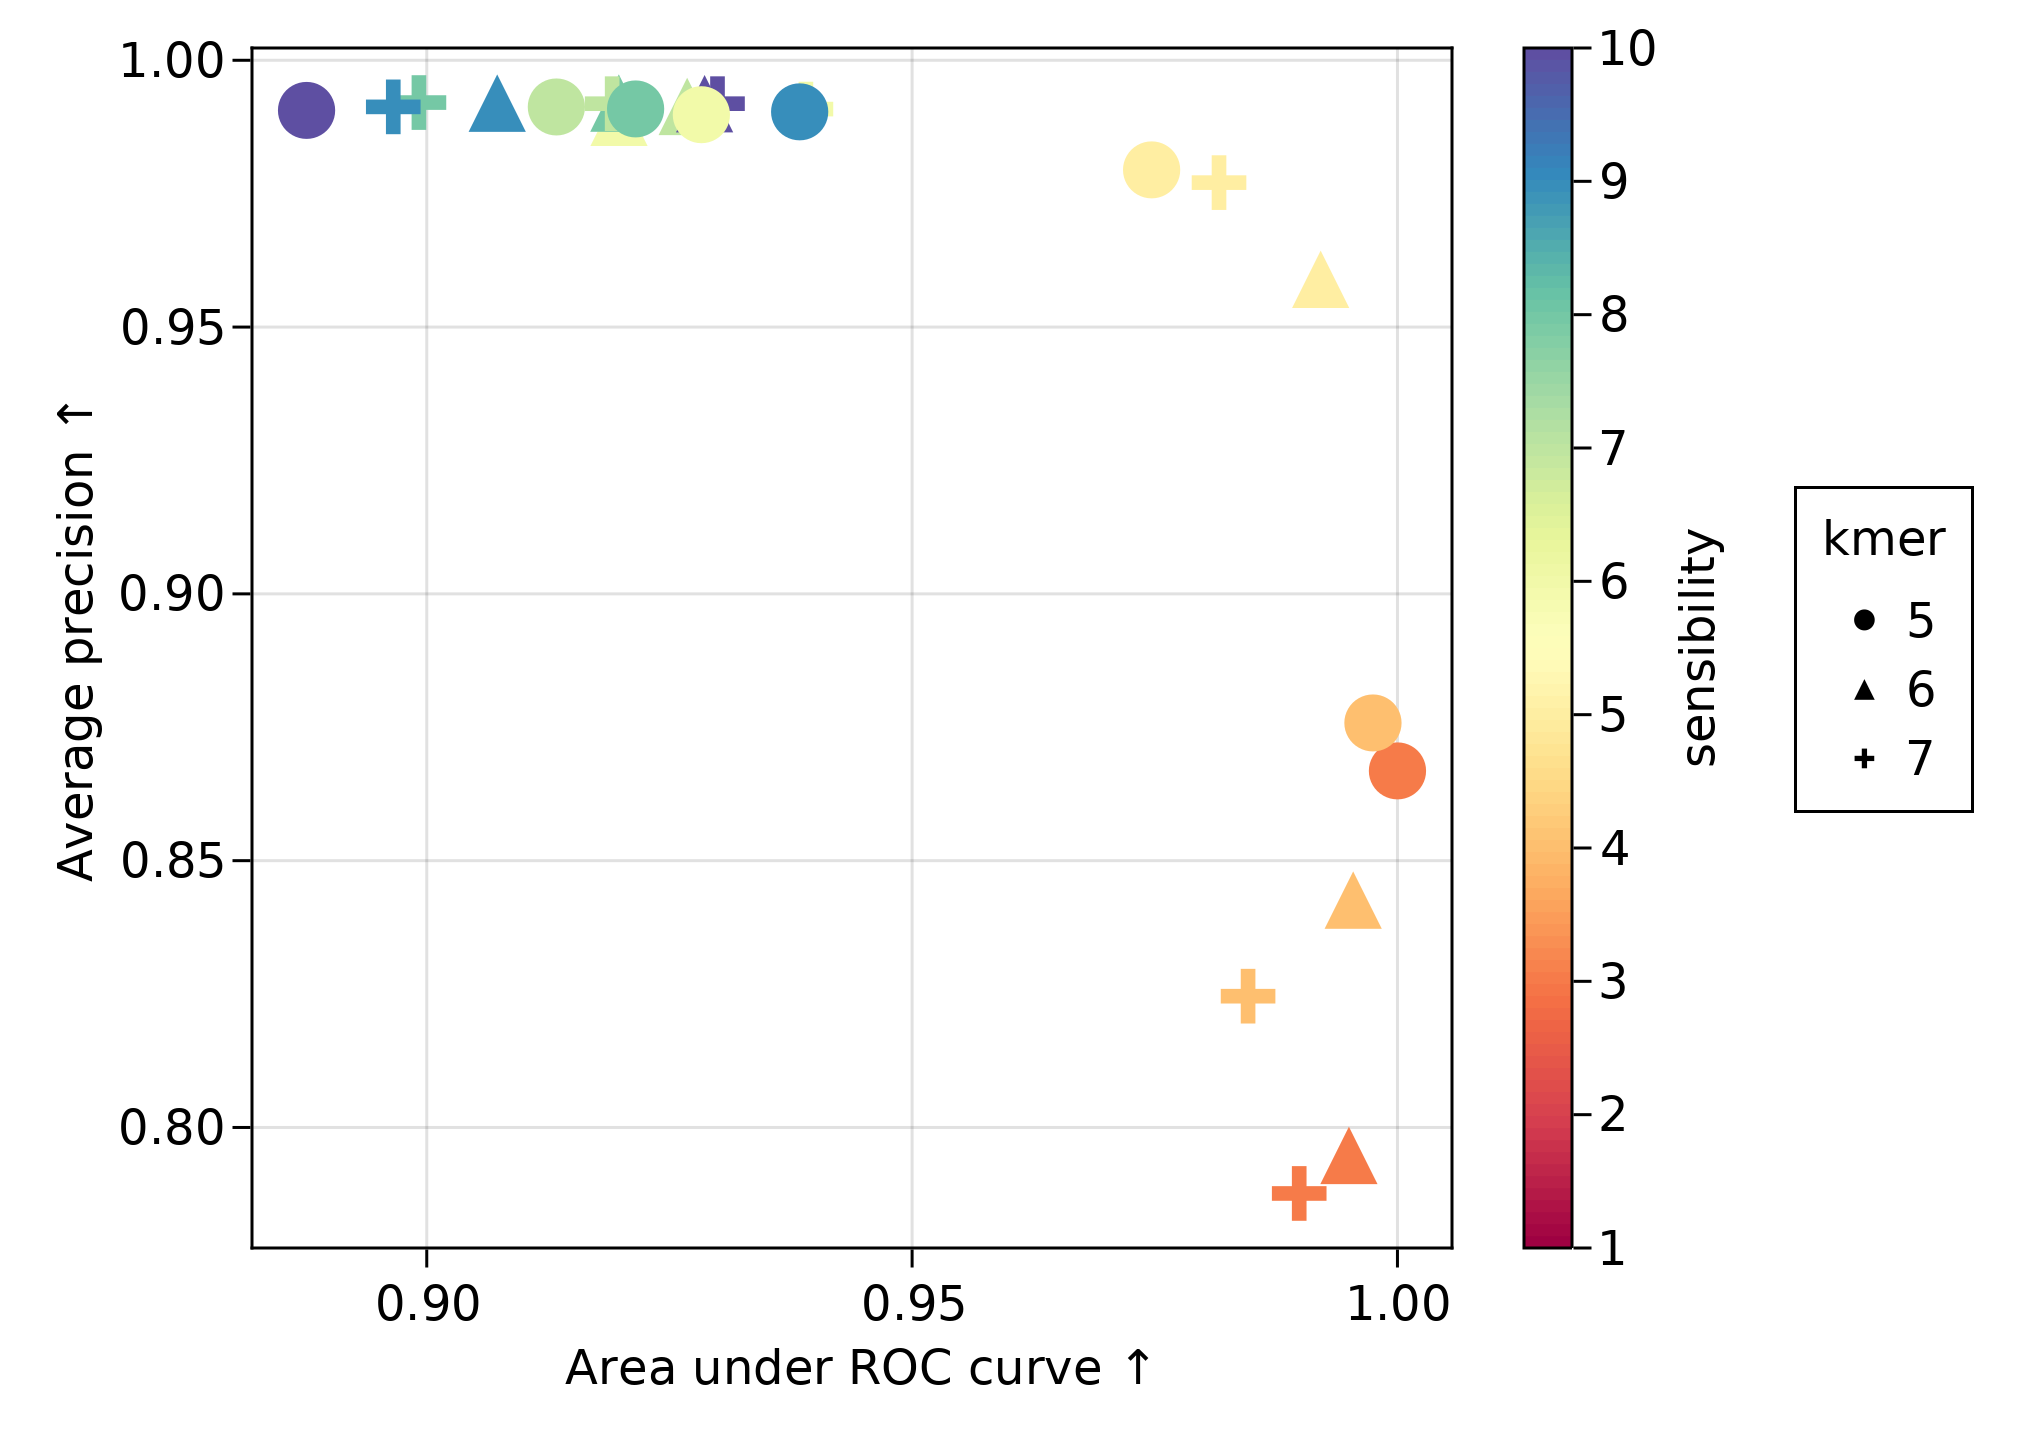
\includegraphics[width=0.8\linewidth]{figures/AuROCvsAuPRC_optimization.png}
	\caption{Parameter optimization for ACE1-like protein search}
	\end{figure}
\end{frame}

\begin{frame}{Results}{\texttt{Foldseek} optimization}
	The optimal parameters for \texttt{Foldseek} for searching for ACE1-like proteins are:
	\begin{itemize}
		\item Sensibility of 5
		\item k-mer size of 5, 6 or 7
	\end{itemize}
\end{frame}

\begin{frame}{Results}{\texttt{Foldseek} exploration}
	\center{Can \texttt{Foldseek} find novel ACE1-like proteins?}
\end{frame}

\begin{frame}{Results}{\texttt{Foldseek} exploration}
	Optimized \texttt{Foldseek}'s parameters for ACE1 protein search:\pause
	\begin{itemize}
		\item Grid-search optimization of \textit{sensibility} \& \textit{k-mer size}\pause 
		\item Complete GO terms used as protein description proxy \pause
		\item Jaccard index of GO terms to assess similarity between proteins \pause
	\end{itemize}

	\bigskip

	\textbf{Objective:} Minimize GO term similarity maintaining performance

\end{frame}

\begin{frame}{Results}{\texttt{Foldseek} exploration}
	\begin{figure}
	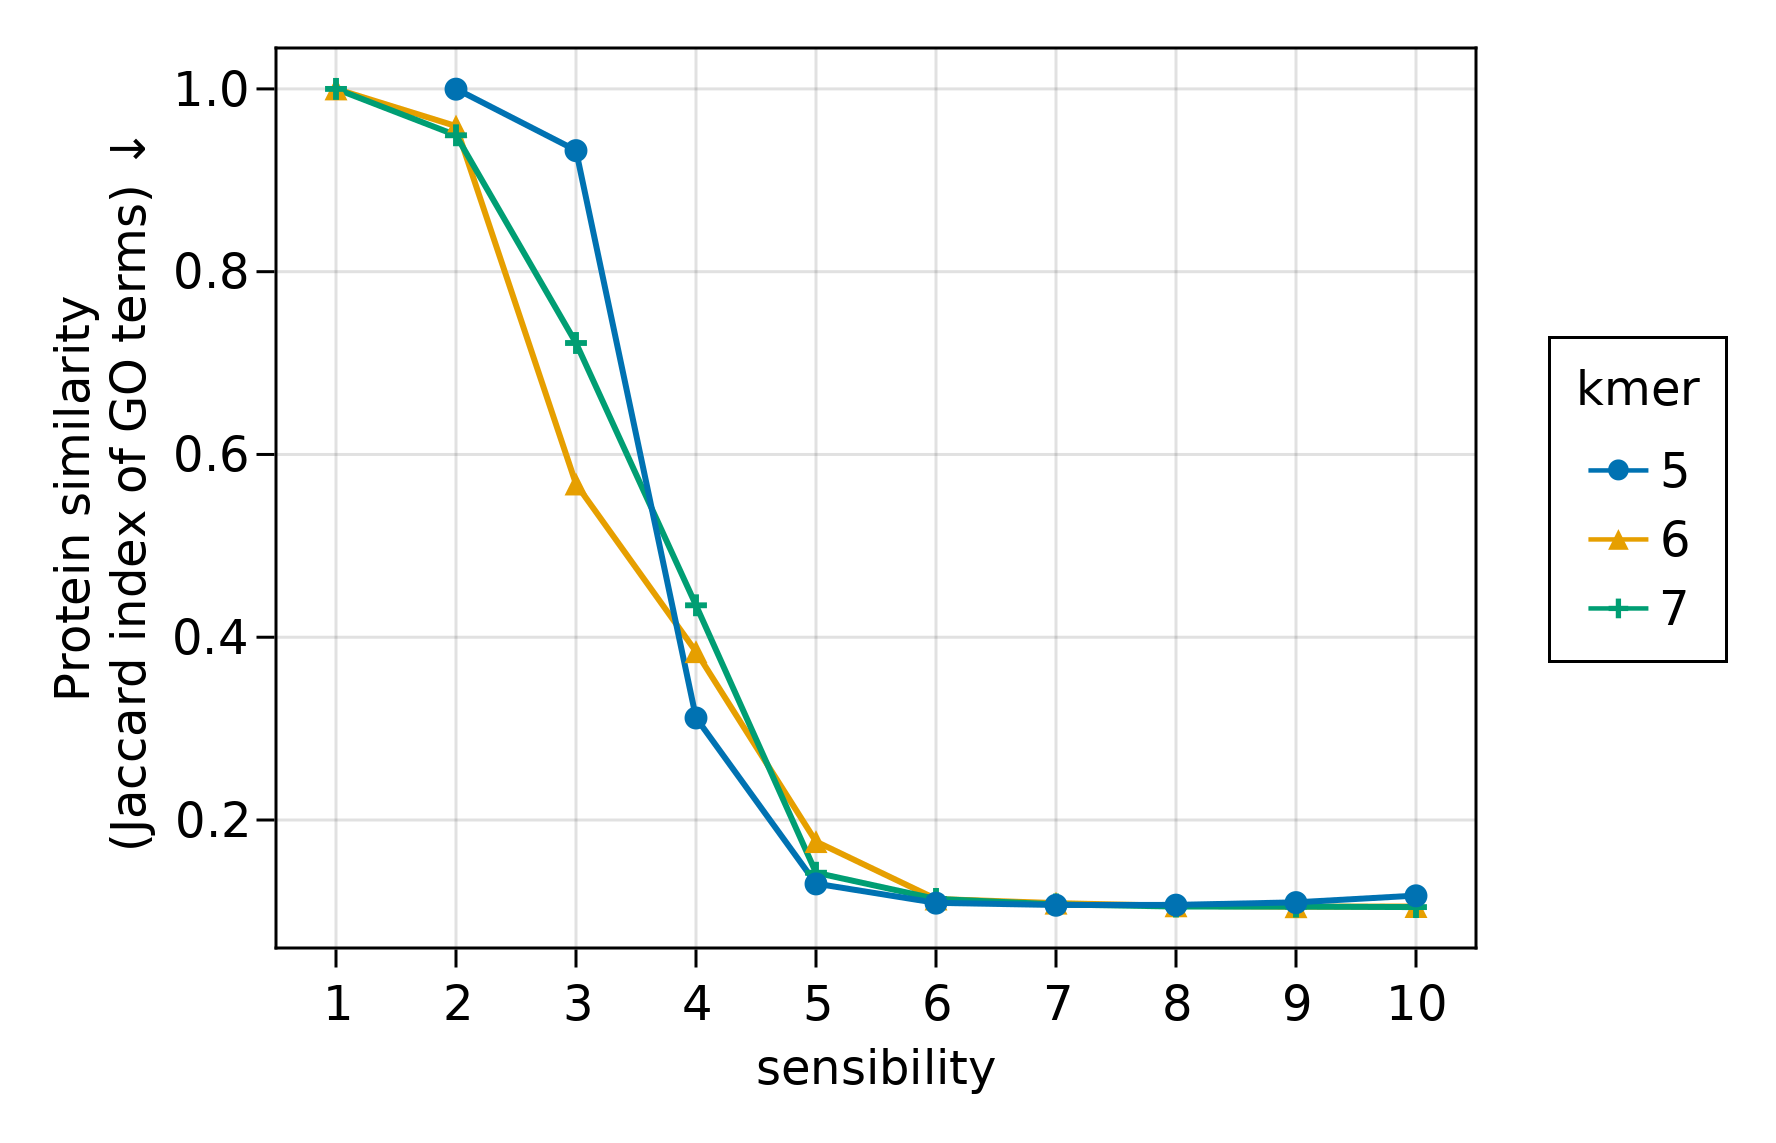
\includegraphics[width=0.8\linewidth]{figures/Jaccard_optimization.png}
	\caption{\texttt{Foldseek} novelty optimization}
	\end{figure}
\end{frame}

\begin{frame}{Results}{\texttt{Foldseek} exploration}
	\begin{figure}
	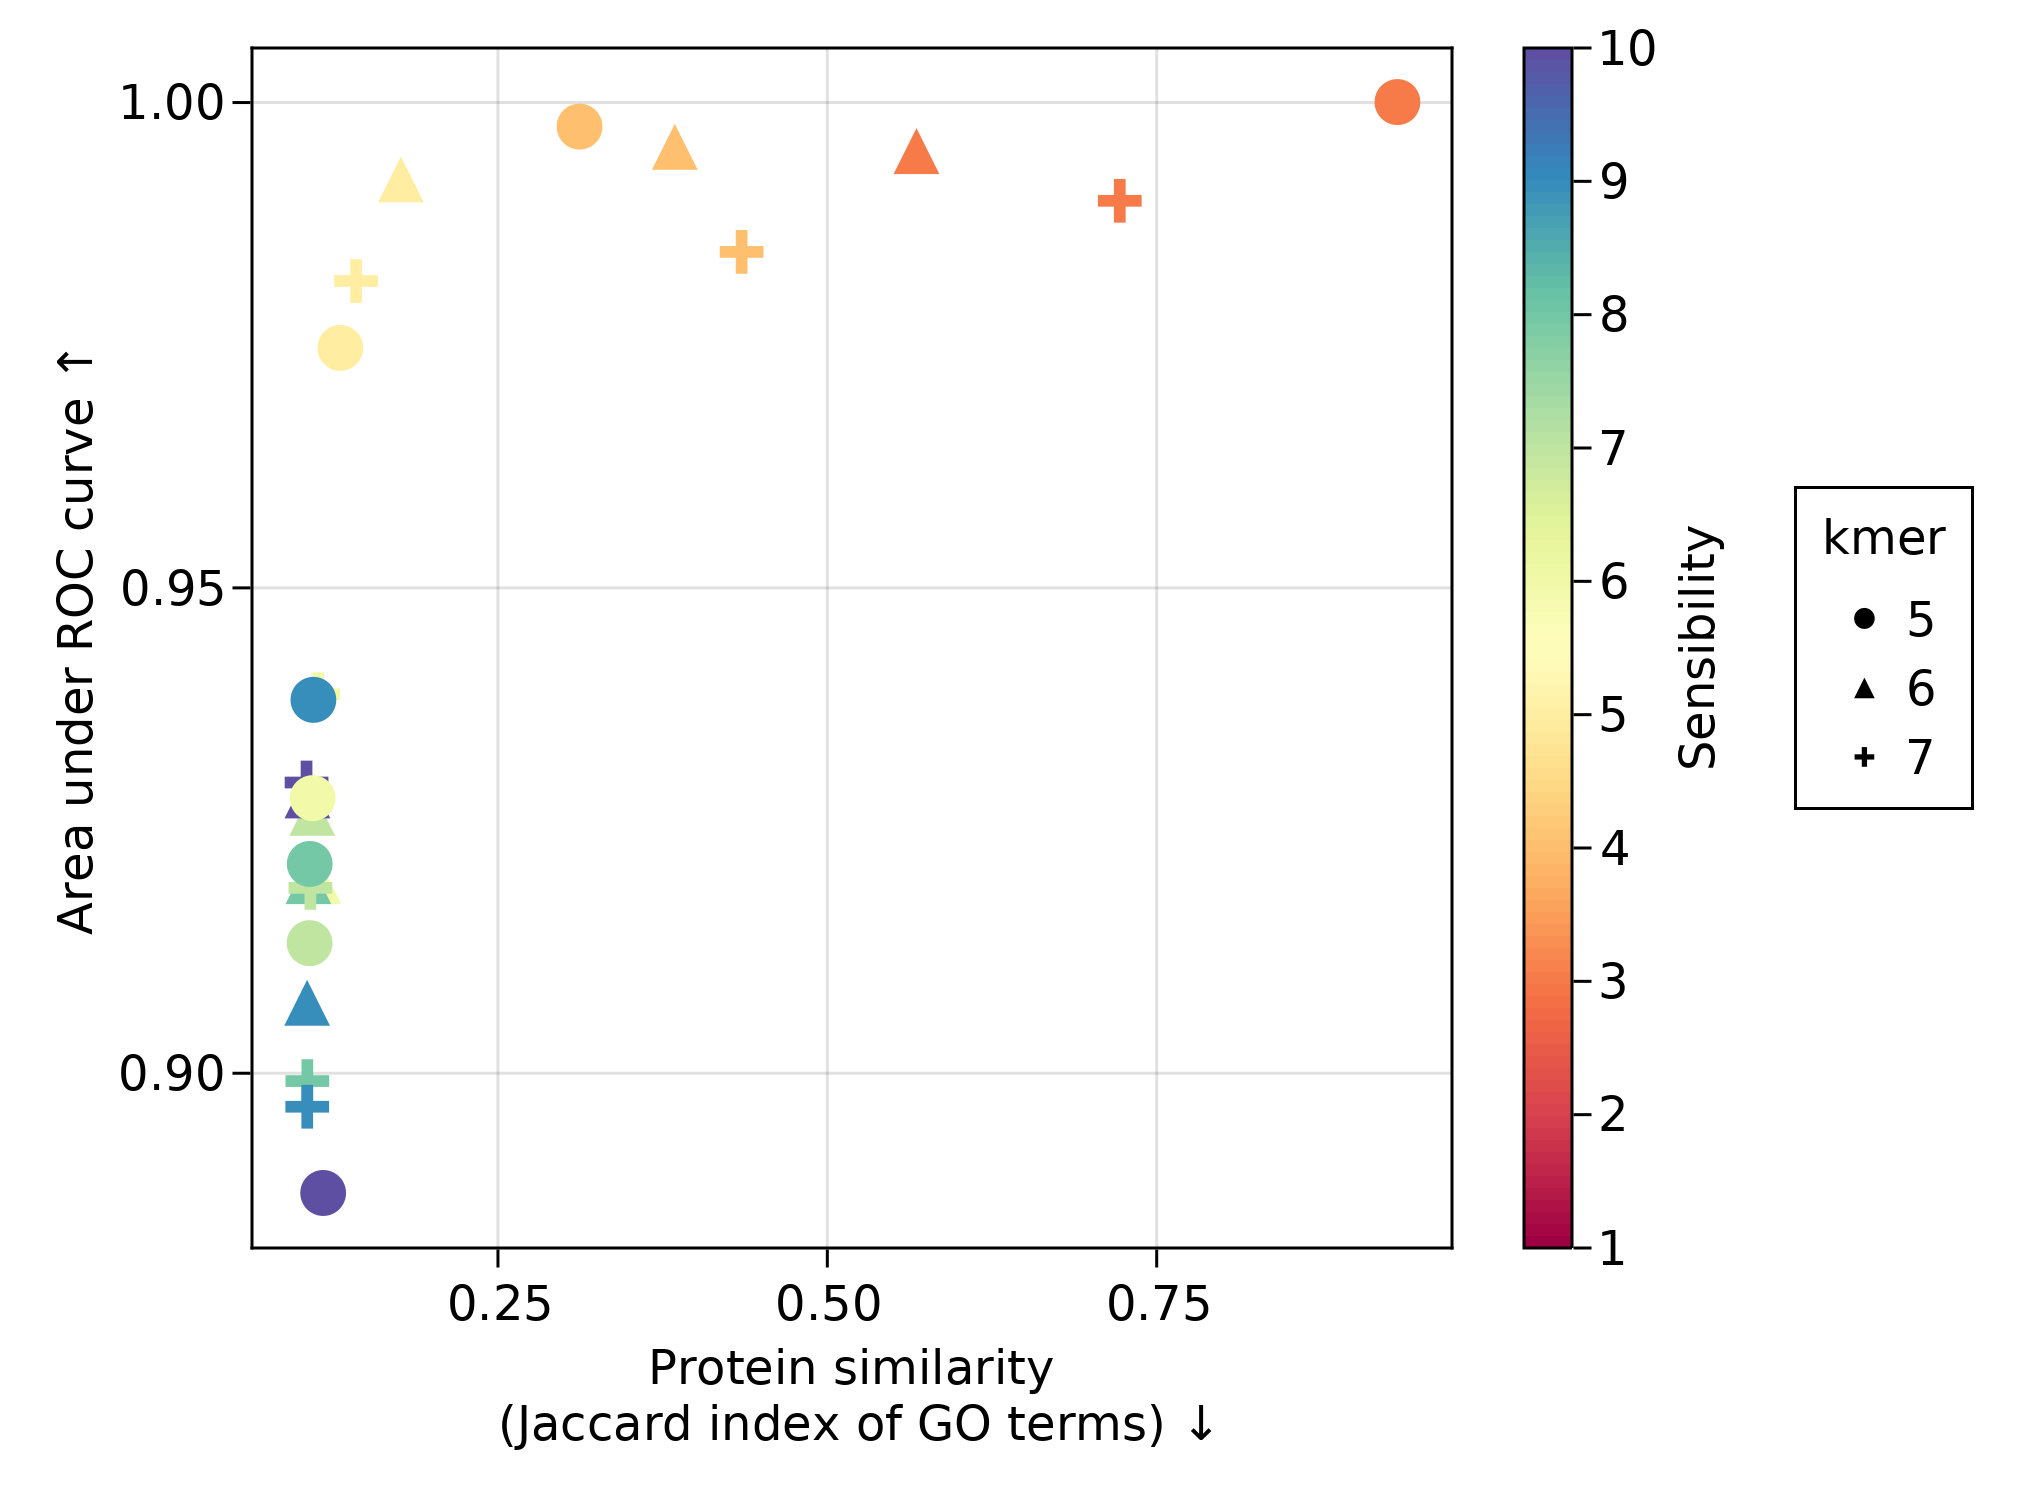
\includegraphics[width=0.8\linewidth]{figures/JaccardvsAuROC_optimization.png}
	\caption{\texttt{Foldseek} novelty optimization as a function of AuROC}
	\end{figure}
\end{frame}

\begin{frame}{Results}{\texttt{Foldseek} exploration}
	\begin{figure}
	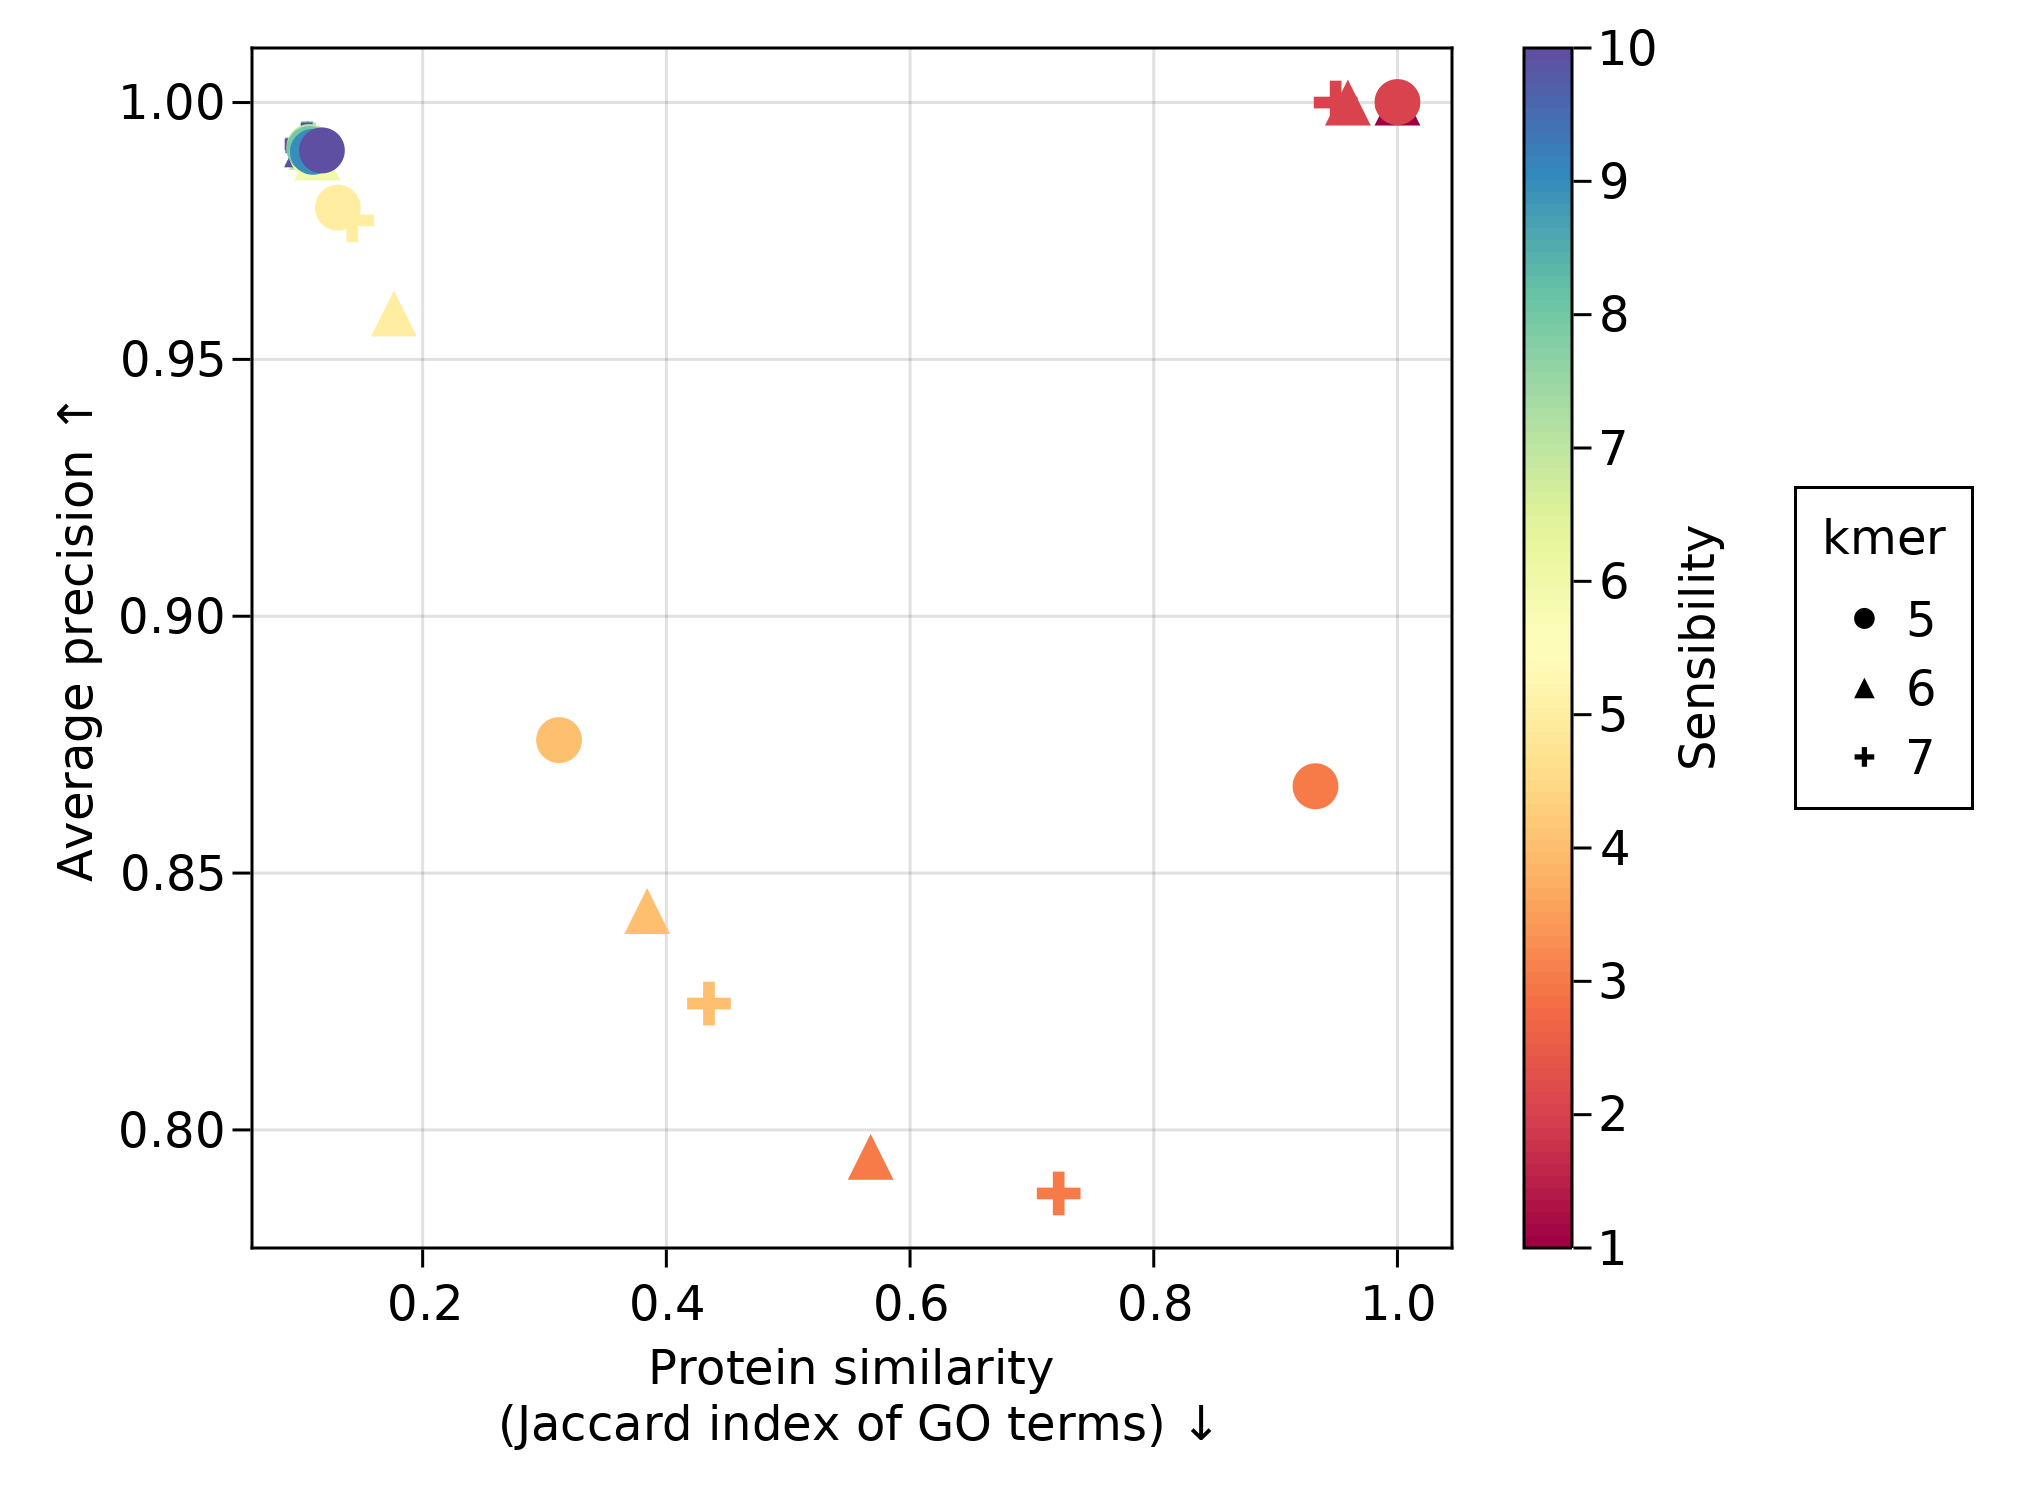
\includegraphics[width=0.8\linewidth]{figures/JaccardvsAuPRC_optimization.png}
	\caption{\texttt{Foldseek} novelty optimization as a function of AuPRC}
	\end{figure}
\end{frame}

\begin{frame}{Results}{\texttt{Foldseek} exploration}
	\begin{figure}
	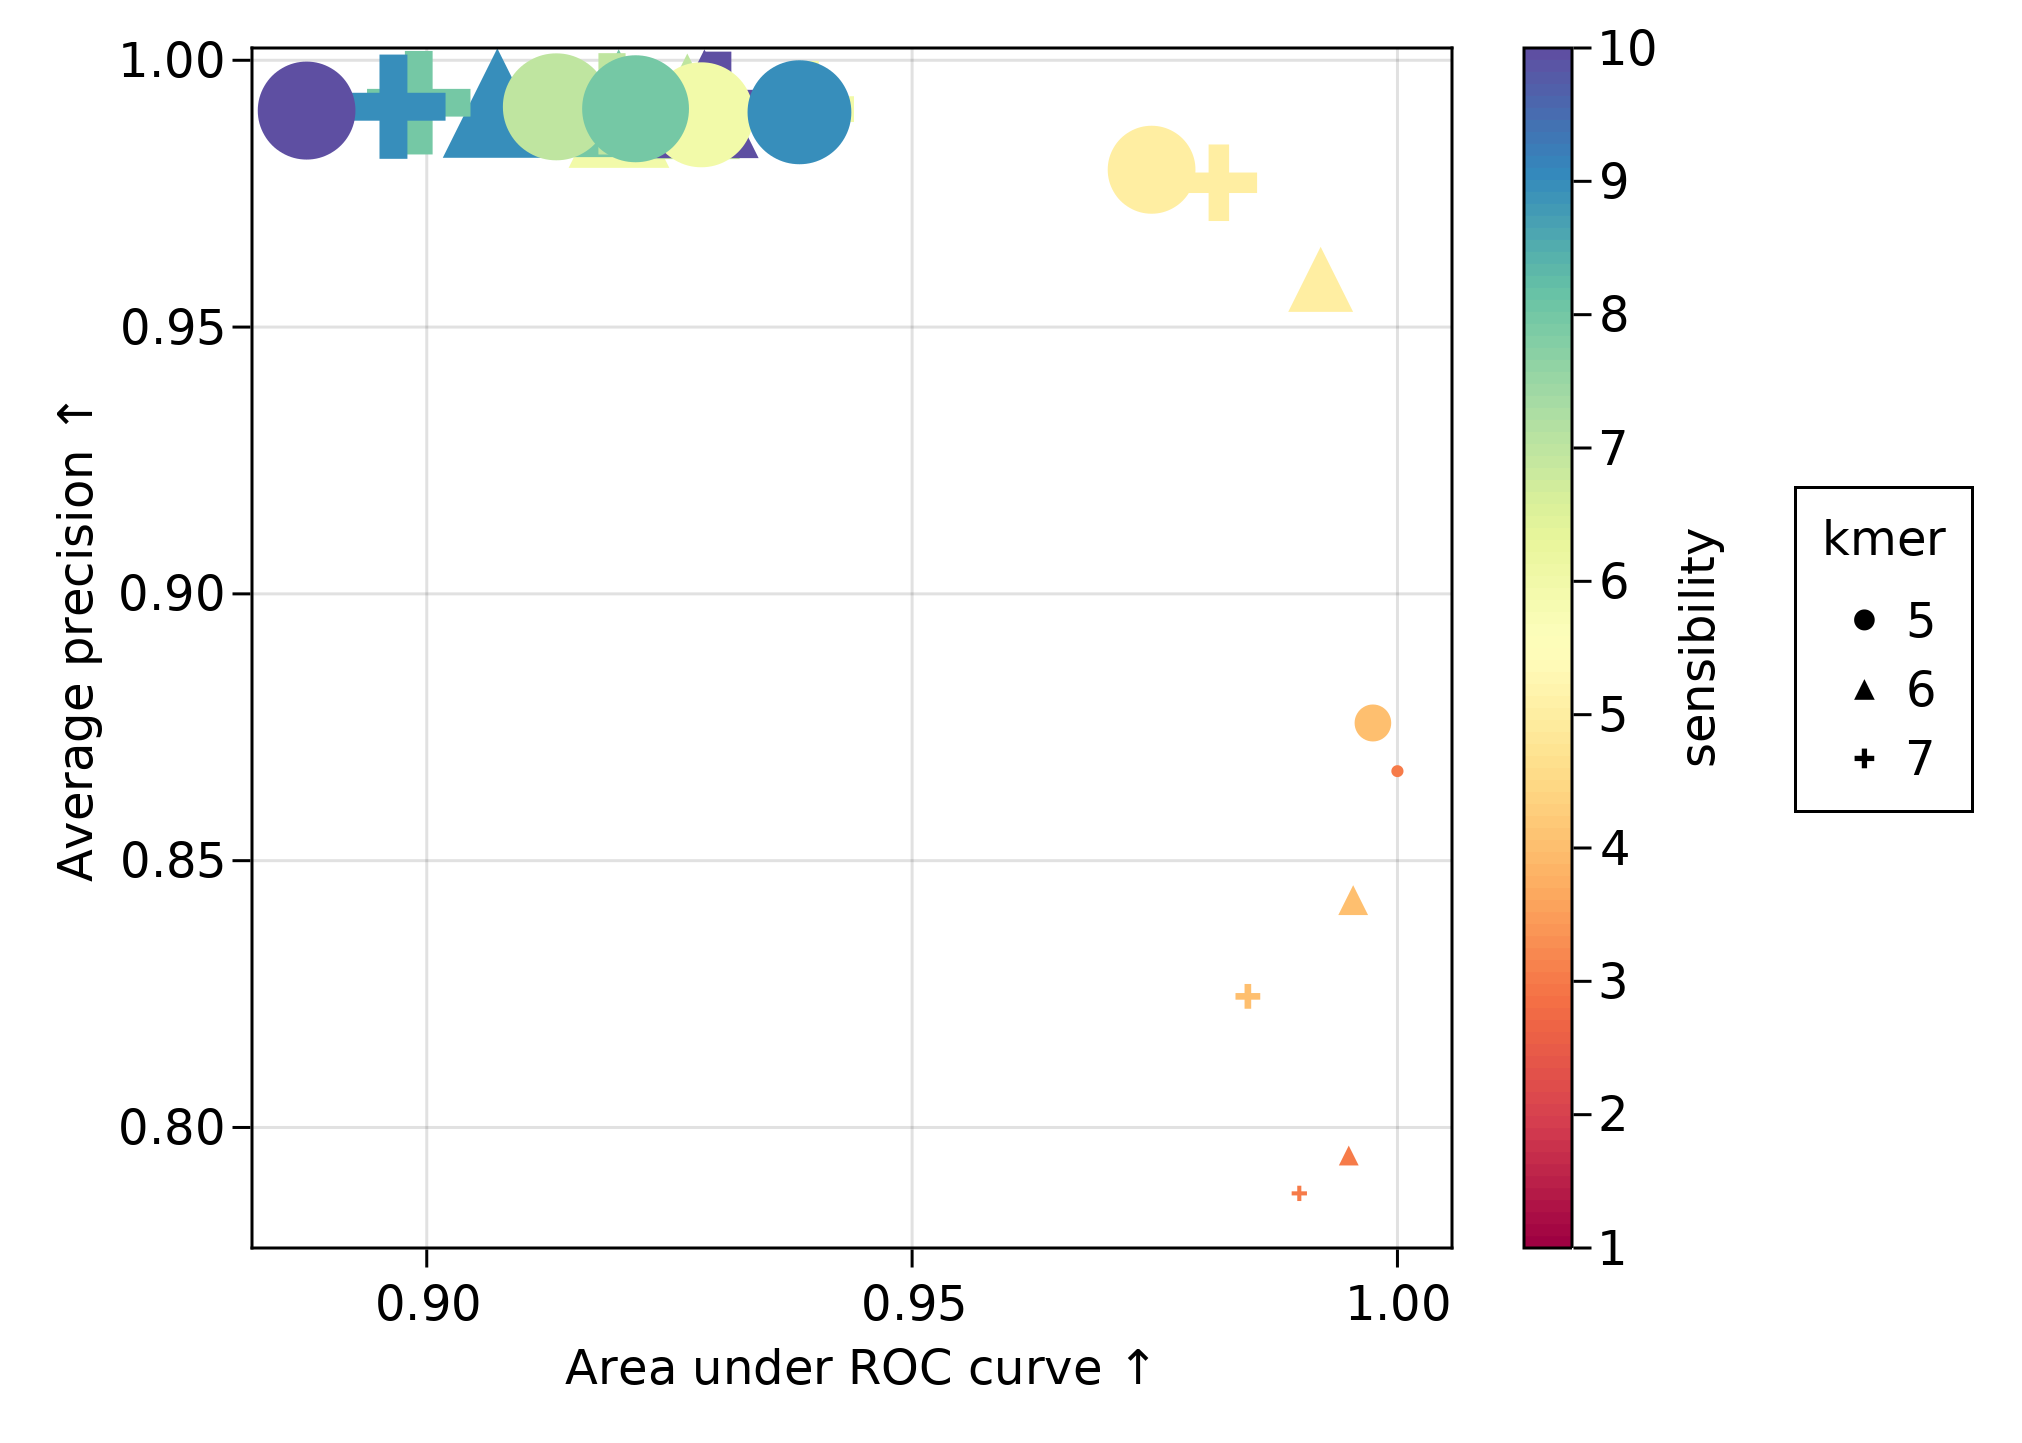
\includegraphics[width=0.8\linewidth]{figures/PerformaceNovelty_optimization.png}
	\caption{\texttt{Foldseek} novelty optimization as a function of AuROC and AuPRC}
	\end{figure}
\end{frame}

\end{document}
